%this file is the first report
%a % comment anything after % until the end of the line

%minimum references to begin our article
\documentclass[12pt]{article}
\usepackage[english]{babel}
\usepackage[utf8]{inputenc}
\usepackage[T1]{fontenc}
\usepackage{graphicx}
\usepackage{fancyhdr}
\usepackage{hyperref}
\usepackage{float}
\usepackage[margin=1in]{geometry}


\pagestyle{fancy}
%\cfoot{Fast and furious game : MonteCarlo drift}
% the last extension makes it possible to add images

%presentation of the document
\title{Fast and furious game : MonteCarlo drift\smallbreak Pre-study and analysis report}
\author{Prateek Bhatnagar, Baptiste Bignon, Mikaïl Demirdelen,\endline Gabriel Prevosto, Dan Seeruttun--Marie,  Benoît Viguier}
\date{10/15/2014}
\begin{document}
\maketitle
\includegraphics[scale=0.5]{img/arimaa}
\newpage
\begin{abstract}
This project is about developing an artificial intelligence for a board game using the \emph{Monte Carlo Tree Search Algorithm} and is coined as \emph{Fast \& Furious Game Playing ,Monte Carlo Drift}. The board game chosen for this project is \emph{Arimaa}.
\newline

\emph{Arimaa} was conceived and developed in 2003 by Umar Syed, a computer science engineer. It was intentionally made difficult for computers to play, while following simple rules. Umar Syed offered a prize of 10000 USD to the first program that can beat a human player in a game of 6 or more matches.
\newline

A revolution in scheduling algorithms originated in the \emph{Monte Carlo Tree Search} algorithm (\emph{MCTS}). \emph{MCTS} is a heuristic search algorithm used for making decisions. It concentrates on analyzing the optimum moves by expansion of a search tree of random samplings called the search space. In this project, the techniques of the \emph{MCTS} algorithm are utilized to find what move to make.
\newline

The program will be implemented using parallelisation techniques, so as to run it on different systems simultaneously. Eventually, the program will be executed on grid 5000, a cluster of multi-core machines.

\end{abstract}


\newpage
%to add a table of contents
\tableofcontents
\newpage

%to create subsections and subsubsubsections, we can use : (chapter n'existe pas avec la classe article)
\section{Presentation of our project}
\subsection{Generalities}
Our project is called Fast and furious game playing, MonteCarlo drift. Our purpose is to create an Artificial Intelligence able to compete against humans using the MonteCarlo Tree Research.
\newline
We will only focus on two players games. Furthermore, we want to avoid games already resolved. We will choose something not studied entirely. We want to work on some new application. That is why we are interested by Arimaa.
\newline
\newline
For our game, we will need a program and statistics to make a good Artificial Intelligence. Each move should be calculated using a reliable method.
MonteCarlo Tree Research is an algorithm able to take these optimal decisions. It has been used in the past for draughts, or chess. By exploring numerous possibilities, it will become possible to know what move is the better one.
We will parallelize this algorithm in order to use it in a multi-core machine, to improve his efficiency.
That MCTS algorithm is better than the classic Min-Max algorithm, that is why we will use it.
\newline
\newline
We will analyse parallelization methods, we will present it, and then we will choose the one adapted to our project.
Thanks to the results of these latest methods, we will be able to choose a state resulting of the current move. Then we will explore the tree and with the same methods as before, we will figure out what the opponent will most probably do. The way we will be exploring the tree will only depend on the parallelization method.
The first part of our project will be the analysis of latest thesis of technologies we will use, in order to choose the best one, and using it on the right environment, to improve his  efficiency.
In the next part, we will choose technologies we will need to achieve our goals, we will create a UML diagram to settle down our program.
\newline
\newline
Finally, in the last part, we will implement this program, and its documentation and test his executing on Grid5000, a cluster of multi-core machines.
What is interesting in this project is we will create an Artificial Intelligence using technologies and methods fully optimized. Then we will create a program that can lead to true improvements for current algorithms applied to this game.



\subsection{Presentation of Arimaa} Arimaa is played on a board composed of 64 tiles, like a chess board. Like in chess, there are 6 types of pieces, but they are not those chess players are used to. From weakest to strongest, they are : rabbits (8 per player), cats, dogs, horses (2 of each per player), camels and elephants (one of each per player).

\begin{figure}[!h]
\centering
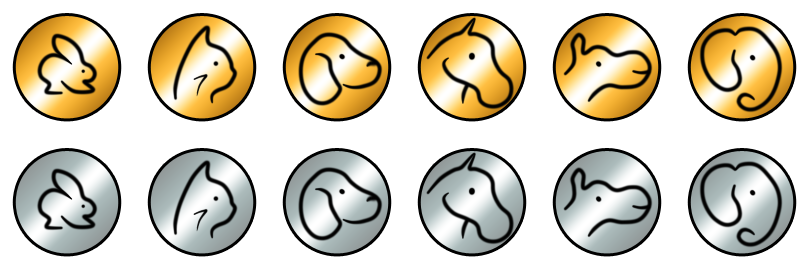
\includegraphics[width=\textwidth]{1_Presentation/1.1_Arimaa_rules_Gabriel/Pictures/Pieces.png}
\caption{\label{fig:pieces}The different piece types in Arimaa.}
\end{figure}

Each player, starting with the gold player, places all of his pieces on the two back rows of his side. Then, the gold player takes the first turn.
On his turn, each player disposes of four moves. He or she can use these moves on a single piece, or on how many pieces as they desire.

All pieces can move on an adjacent square (but not diagonally), except for the rabbit which cannot move backwards.
A piece can instead use two moves to push or pull a weaker adjacent enemy piece, as shown in \ref{fig:displace}.

\begin{figure}[!h]
\centering
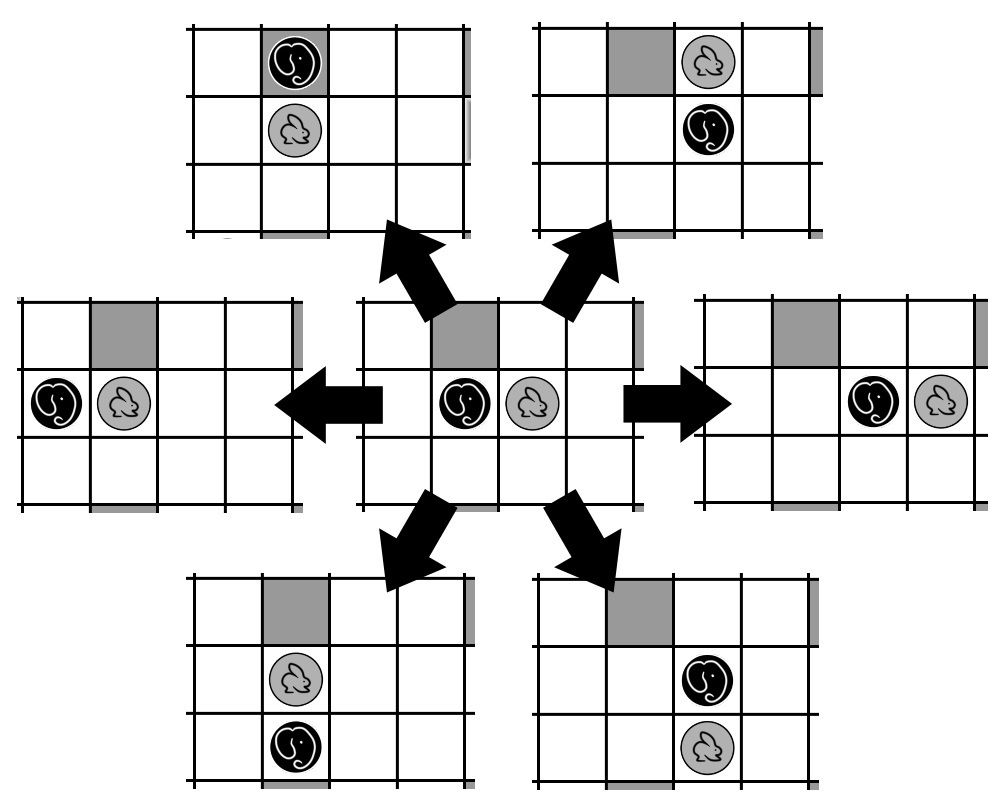
\includegraphics[width=0.5\textwidth]{1_Presentation/1.1_Arimaa_rules_Gabriel/Pictures/Displace.png}
\caption{\label{fig:displace}The different ways you can push or pull a weaker enemy piece.}
\end{figure}

A piece sitting next to a stronger enemy piece is frozen. When a piece is frozen, it cannot move. As shown in figure \ref{fig:freeze}, a piece cannot be frozen while there is an ally piece beside it.

\begin{figure}[!h]
\centering
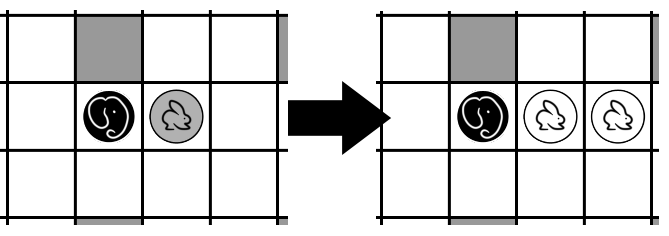
\includegraphics[width=0.5\textwidth]{1_Presentation/1.1_Arimaa_rules_Gabriel/Pictures/Freeze.png}
\caption{\label{fig:freeze}Example of the freezing mechanic.}
\end{figure}

There are four traps on the board. As shown in figure \ref{fig:trap}, any piece sitting on a trap with no ally piece next to it dies.

\begin{figure}[!h]
\centering
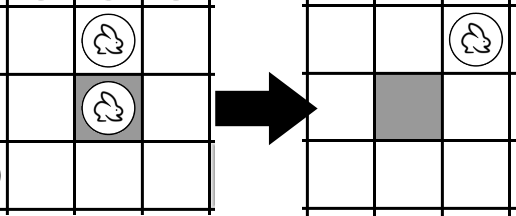
\includegraphics[width=0.5\textwidth]{1_Presentation/1.1_Arimaa_rules_Gabriel/Pictures/Trap.png}
\caption{\label{fig:trap}Example of the traps mechanic.}
\end{figure}

There are three ways to win the game :

\begin{description}
\item[Victory by reaching the goal] You win the game if one of your rabbits reaches the other end of the board.
\item[Victory by elimination] You win the game if you eliminate all the rabbits belonging to the opponent.
\item[Victory by elimination] You win the game if the opponent can't make a move on his turn.
\item[Victory by repetition] If the same position happens three times in a row, the player that makes it happen the third time loses the game.
\end{description}
\section{Algorithms}\subsection{The Minimax algorithm}
% miss the blank space
The Minimax algorithm is a way of finding an optimal move in a two player game. In the search tree for a two player game, there are two kinds of nodes, nodes representing ones moves and nodes representing the opponent's moves.\cite{graphics_minimax}
\begin{figure}[H]
\centering
	\begin{minipage}[b]{0.45\linewidth}
		\centering
		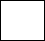
\includegraphics[height=1cm]{2_State_of_the_art/Arimaa_on_MCTS_Benoit/img/max.png}
		\caption{\label{fig:max}Nodes representing ones moves are generally drawn as squares, these are also called \emph{MAX} nodes.}
	\end{minipage}%
	\hspace*{1cm}
	\begin{minipage}[b]{0.45\linewidth}
		\centering
		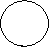
\includegraphics[height=1cm]{2_State_of_the_art/Arimaa_on_MCTS_Benoit/img/min.png}
		\caption{\label{fig:min}Nodes representing the opponent's moves are generally drawn as circles, these are also called \emph{MIN} nodes.}
	\end{minipage}%
\end{figure}

The goal of a \emph{MAX/MIN} node is to maximize/minimize the value of the subtree rooted at that node. To do this, a \emph{MAX/MIN} node chooses the child with the greatest/smallest value, and that becomes the value of the \emph{MAX/MIN} node.

Note that it's typical for two player games to have different branching factors at each node. The move one makes could have an impact on what moves are possible for the opponent. In this example, one is ignoring what the game is in order to focus on the algorithm.

\begin{figure}[H]
\centering
	\begin{minipage}[b]{0.45\linewidth}
		\centering
		\includegraphics[height=1.5cm]{2_State_of_the_art/Arimaa_on_MCTS_Benoit/img/Minimax2.png}
		\caption{\label{fig:Minimax2}At the start of the problem, Minimax checks the single present node.}
	\end{minipage}%
	\hspace*{1cm}
	\begin{minipage}[b]{0.45\linewidth}
		\centering
		\includegraphics[height=3cm]{2_State_of_the_art/Arimaa_on_MCTS_Benoit/img/Minimax3.png}
		\caption{\label{fig:Minimax3}It begins like a depth first search, generating the first child.}
	\end{minipage}%
\end{figure}

So far we've really seen no evaluation values. The way Minimax works is to go down a specified number of full moves (where one \emph{full move}' is actually a move by each player), then calculate the evaluation values for states at that depth. For this example, we're going to go down one full move, which is one more level.
\begin{figure}[H]
\centering
	\begin{minipage}[b]{0.45\linewidth}
		\centering
		\includegraphics[height=3cm]{2_State_of_the_art/Arimaa_on_MCTS_Benoit/img/Minimax4.png}
		\caption{\label{fig:Minimax4}we generate the values for those nodes.}
	\end{minipage}%
	\hspace*{1cm}
	\begin{minipage}[b]{0.45\linewidth}
		\centering
		\includegraphics[height=3cm]{2_State_of_the_art/Arimaa_on_MCTS_Benoit/img/Minimax5.png}
		\caption{\label{fig:Minimax5}It chooses the minimum of the two child node values, which is 3.}
	\end{minipage}%
\end{figure}

The max node at the top still has two other children nodes that we need to generate and search.

\begin{figure}[H]
\centering
	\begin{minipage}[b]{0.45\linewidth}
		\centering
		\includegraphics[height=3cm]{2_State_of_the_art/Arimaa_on_MCTS_Benoit/img/Minimax6.png}
		\caption{\label{fig:Minimax6}Since there is only one child, the min node must take it's value.}
		\end{minipage}%
	\hspace*{1cm}
	\begin{minipage}[b]{0.45\linewidth}
		\centering
		\includegraphics[height=3cm]{2_State_of_the_art/Arimaa_on_MCTS_Benoit/img/Minimax8.png}
		\caption{\label{fig:Minimax8}The third min node chooses the minimum of it's child node values, 1.}
	\end{minipage}%
\end{figure}

Finally we have all of the values of the children of the max node at the top level, so it chooses the maximum of them, 15, and we get the final solution. 

\begin{figure}[H]
\centering
	\begin{minipage}[b]{1\linewidth}
		\centering
		\includegraphics[height=3cm]{2_State_of_the_art/Arimaa_on_MCTS_Benoit/img/Minimax9.png}
		\caption{\label{fig:Minimax9}Final tree.}
	\end{minipage}%
\end{figure}

What this tells us is that we should take the move that leads to the middle min node, since it'll lead to the best possible state for us one full move down the road.

\subsection{The \ensuremath{\alpha\beta} pruning} %pruning = elaguage en anglais
The \ensuremath{\alpha\beta} method is a heuristic that decrease the number of leaf that will be explored by the Minimax algorithm. That way, the size of the tree will be smaller, the algorithm will be able to dive further and the time spend on more interesting subtree is greater.\\
If the leaf's position is less interesting than its parents, the algorithm won't explore anyfurther.

\subsection{Monte Carlo Tree Search Algorithm}
\subsubsection{Introduction}
Monte Carlo Tree Search (MCTS) is an algorithm used for taking decisions in Artificial Intelligence (AI) problems such as solving games or decision making in project managment. It is based on making a big number of random simulations in order to get trustfull datas. To make such simulations, the program play the moves randomly for each players. Once it reach a conclusion (win or loss), the program compute the statistics to get the odds of winning.
\subsubsection{How does it works ?}
The Algorithm create a tree with all possible solution with a small depth.
Then it start to run random simulations starting from the leaves in order to test the odds of the outcome.
Once we got enough the results (usually we are using time based simulations) we feed back the results and make the decision depending on the odds of each subsequent leaves.
\subsubsection{Example}
\label{sec:example}
\begin{figure}[H]
\centering
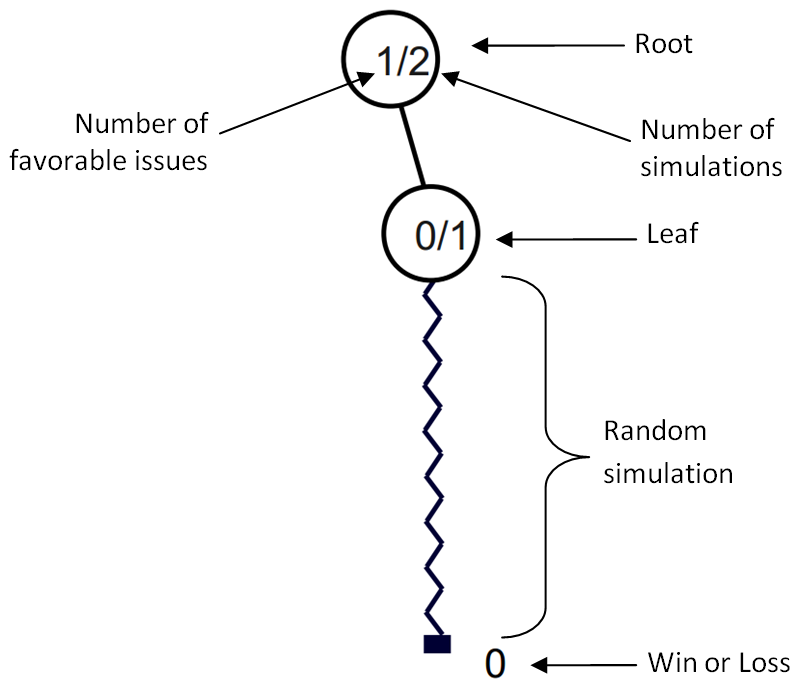
\includegraphics[height=5cm]{1_Presentation/1.2_Algorithm_MCTS_Benoit/img/schema.png}
\caption{\label{fig:schema}Legend of the following figures.}
\end{figure}

\begin{figure}[H]
\centering
	\begin{minipage}[b]{0.45\linewidth}
		\centering
		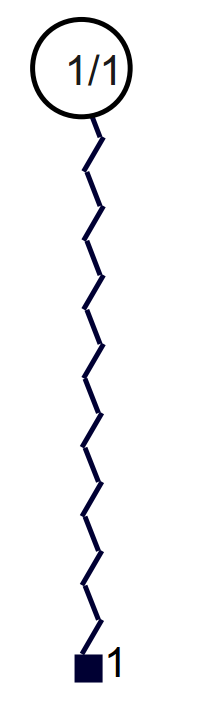
\includegraphics[height=4cm]{1_Presentation/1.2_Algorithm_MCTS_Benoit/img/1.png}
		\caption{\label{fig:1}Run a first simulation from the root, get a favorable issue (will be considered as a \textit{win}).}
	\end{minipage}%
	\hspace*{1cm}
	\begin{minipage}[b]{0.45\linewidth}
		\centering
		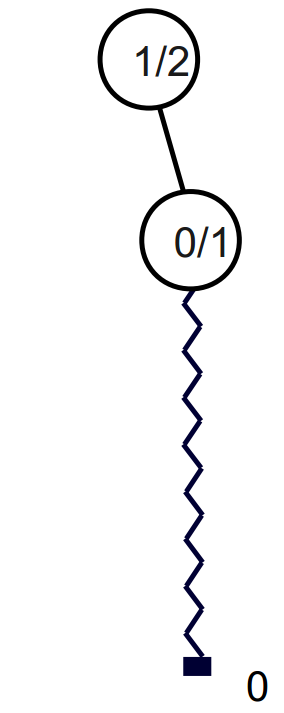
\includegraphics[height=4cm]{1_Presentation/1.2_Algorithm_MCTS_Benoit/img/2.png}
		\caption{\label{fig:2}Create a first leaf at depth 1 and run the simulation, get an unfavorable issue (considered as a \textit{loss}).}
	\end{minipage}%
\end{figure}

\begin{figure}[H]
\centering
	\begin{minipage}[b]{0.3\linewidth}
		\centering
		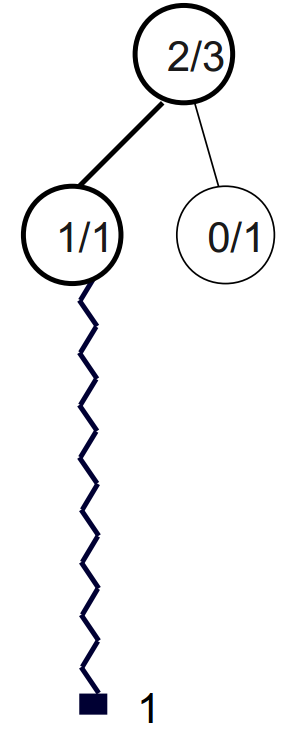
\includegraphics[height=4cm]{1_Presentation/1.2_Algorithm_MCTS_Benoit/img/3.png}
		\caption{\label{fig:3}Create a second leaf at depth 1 and run the simulation (\textit{win}).}
	\end{minipage}%
	\hspace*{1cm}
	\begin{minipage}[b]{0.3\linewidth}
		\centering
		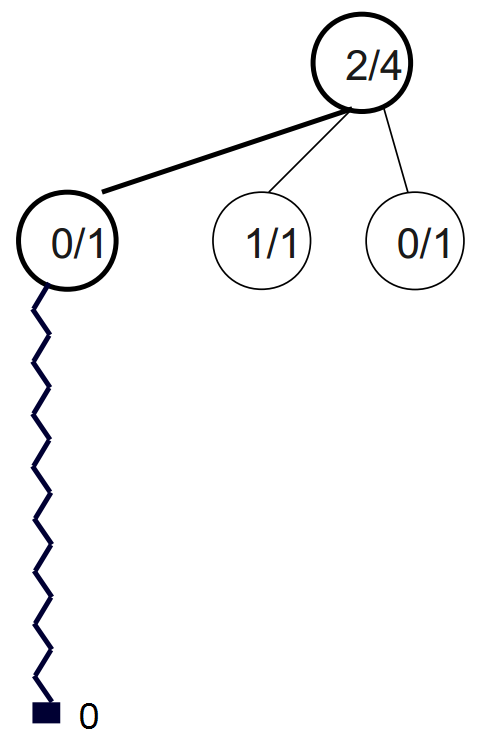
\includegraphics[height=4cm]{1_Presentation/1.2_Algorithm_MCTS_Benoit/img/4.png}
		\caption{\label{fig:4}Create a third leaf at depth 1 and run the simulation (\textit{loss}).}
	\end{minipage}%
	\hspace*{1cm}
	\begin{minipage}[b]{0.3\linewidth}
		\centering
		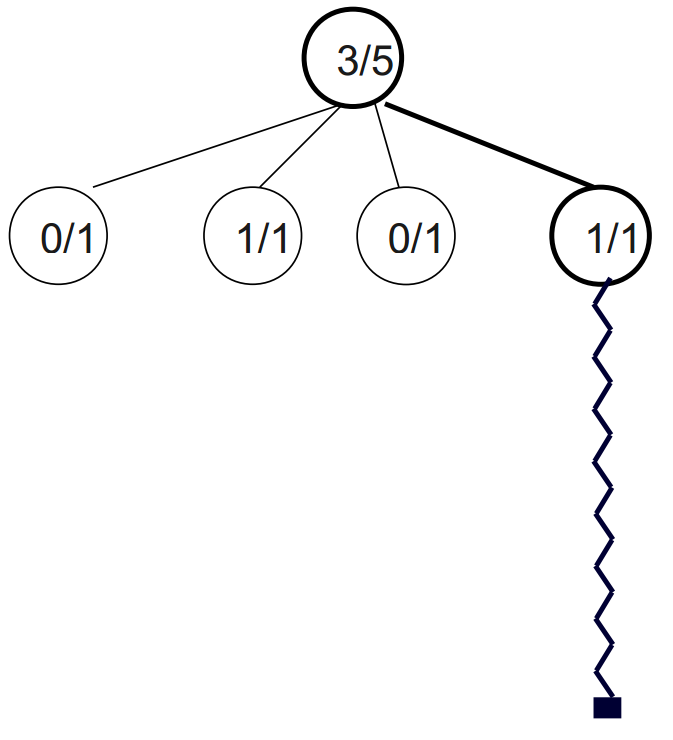
\includegraphics[height=4cm]{1_Presentation/1.2_Algorithm_MCTS_Benoit/img/5.png}
		\caption{\label{fig:5}Create a fourth leaf at depth 1 and run the simulation (\textit{win}).}
	\end{minipage}%
\end{figure}

Right now the odds of winning are 3/5. Now that we tested all the possible outcomes at depth 1, we will expend the tree on the favorable leaves (here the second and fourth).

\begin{figure}[H]
\centering
	\begin{minipage}[b]{0.45\linewidth}
		\centering
		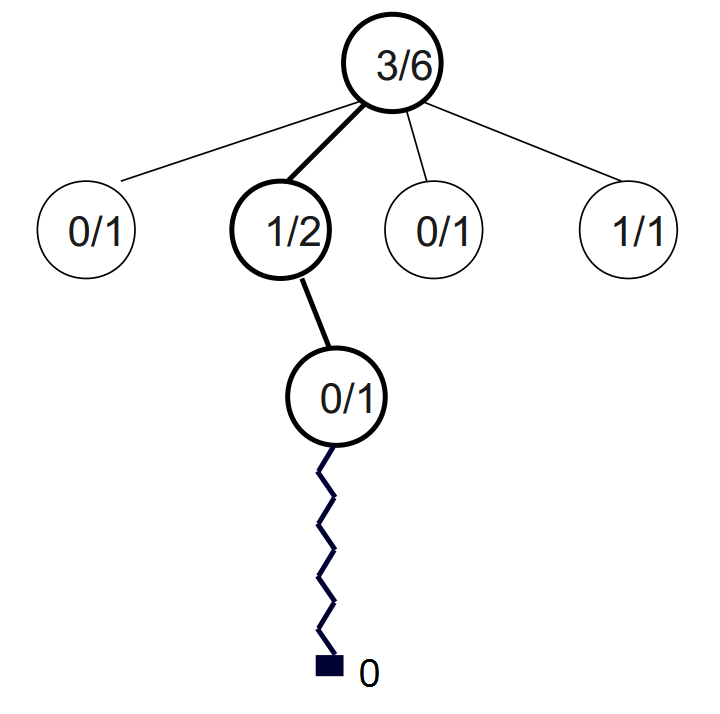
\includegraphics[height=4cm]{1_Presentation/1.2_Algorithm_MCTS_Benoit/img/6.png}
		\caption{\label{fig:6}Create a leaf at depth 2 with parent the 2nd leaf at depth 1 and run the simulation (\textit{loss}), update the odds value of the node and making it less interesting than the fourth node. Therefore the algorithm will now work on the fourth node.}
	\end{minipage}%
	\hspace*{1cm}
	\begin{minipage}[b]{0.45\linewidth}
		\centering
		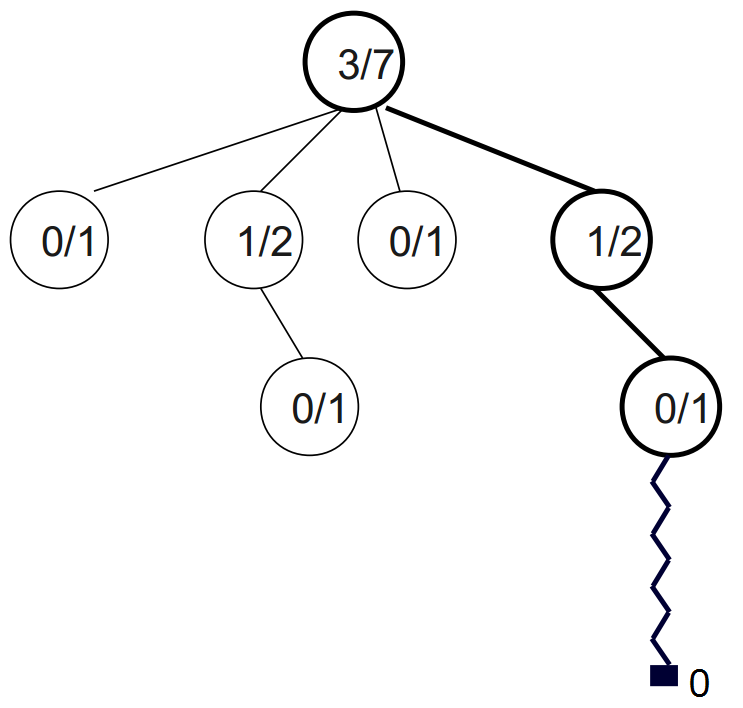
\includegraphics[height=4cm]{1_Presentation/1.2_Algorithm_MCTS_Benoit/img/7.png}
		\caption{\label{fig:7}Create a leaf at depth 2 with parent the fourth leaf at depth 1 and run the simulation (\textit{loss}), update the odds value of the node and making it as interesting as the second node. The algorithm will now work on the second node.}
	\end{minipage}%
\end{figure}
\begin{figure}[H]
\centering
	\begin{minipage}[b]{0.45\linewidth}
		\centering
		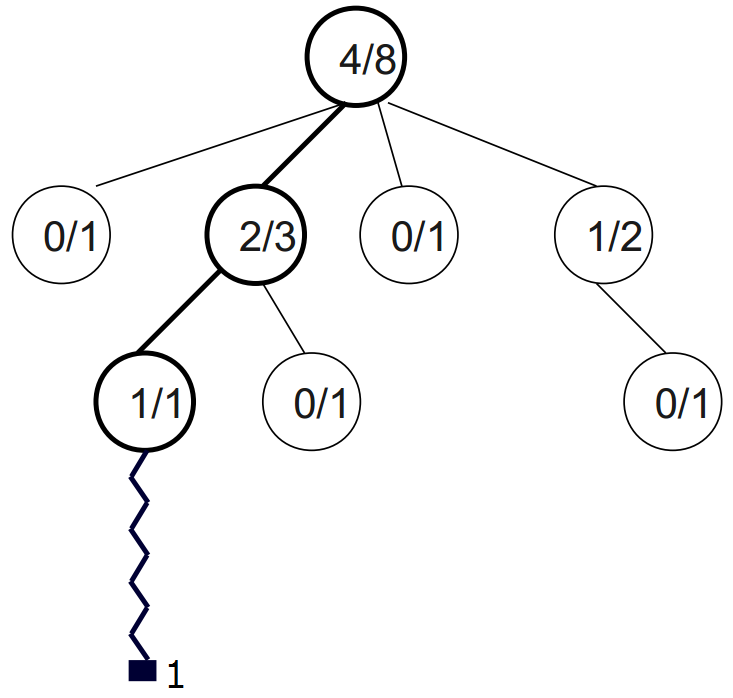
\includegraphics[height=4cm]{1_Presentation/1.2_Algorithm_MCTS_Benoit/img/8.png}
		\caption{\label{fig:8}Create a second leaf at depth 2 with parent the second leaf at depth 1 and run simulation (\textit{win}), update the odds value and continue to develop this leaf.}
	\end{minipage}%
	\hspace*{1cm}
	\begin{minipage}[b]{0.45\linewidth}
		\centering
		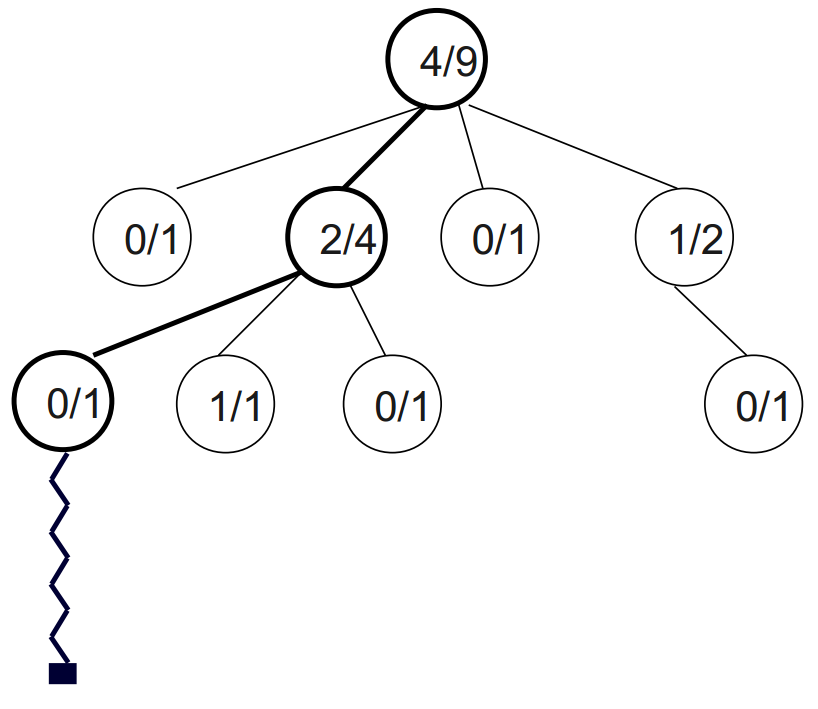
\includegraphics[height=4cm]{1_Presentation/1.2_Algorithm_MCTS_Benoit/img/9.png}
		\caption{\label{fig:9}Create a third leaf at depth 2 with parent the second leaf at depth 1 and run simulation (\textit{loss}), update the odds value and switch to the fourth leaf.\null\\}
	\end{minipage}%
\end{figure}

Continue the Algorithm until a decent about of simulation are run and/or the time limit is .
\begin{figure}[H]
\centering
	\begin{minipage}[b]{0.33\linewidth}
	\centering
		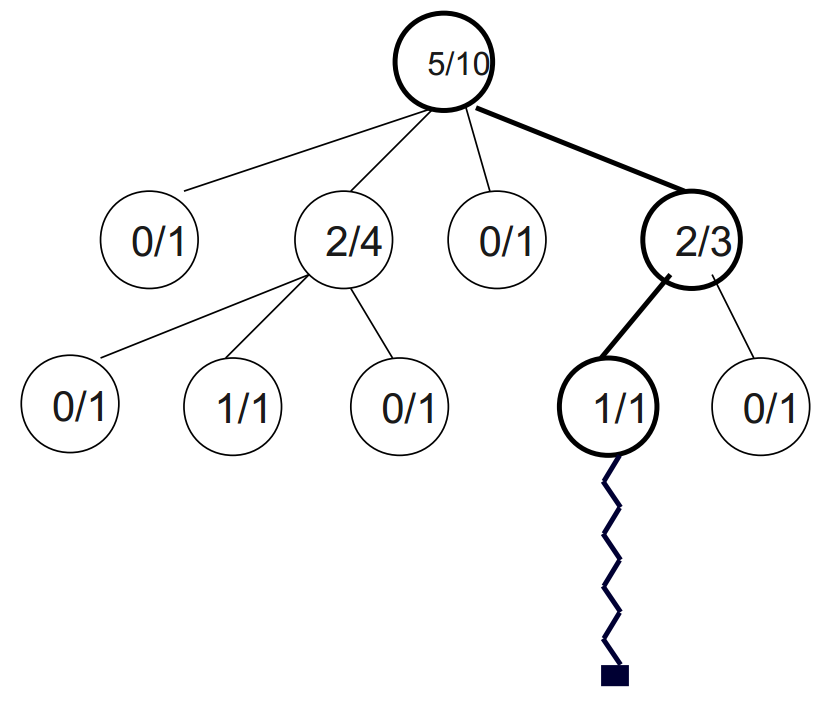
\includegraphics[height=4cm]{1_Presentation/1.2_Algorithm_MCTS_Benoit/img/10.png}
	\end{minipage}%
	\begin{minipage}[b]{0.33\linewidth}
	\centering
		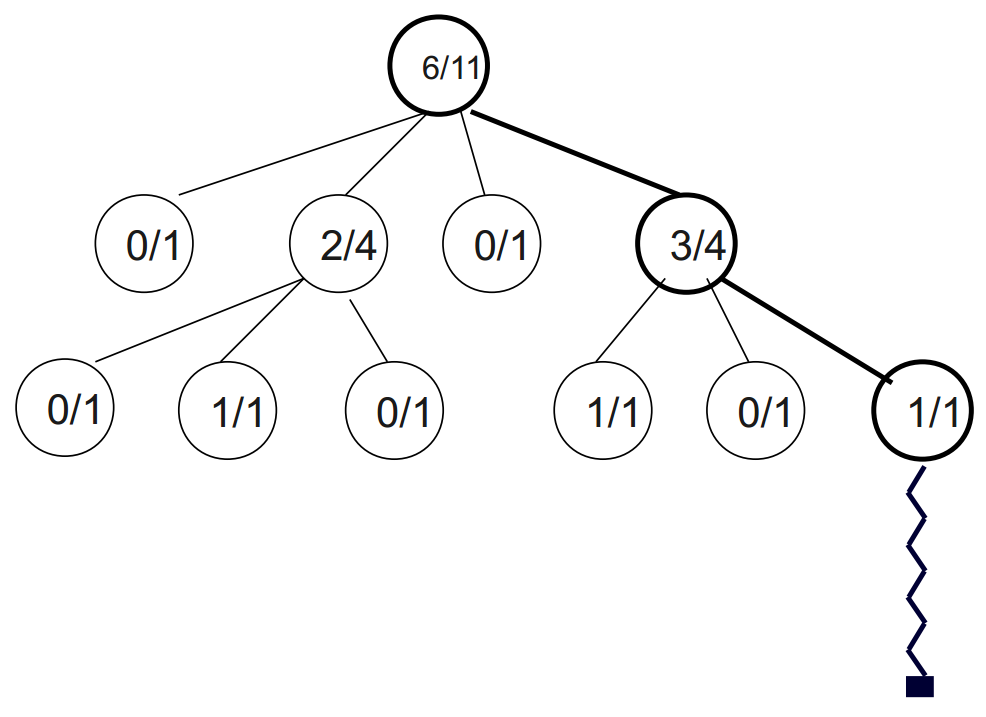
\includegraphics[height=4cm]{1_Presentation/1.2_Algorithm_MCTS_Benoit/img/11.png}
	\end{minipage}%
	\begin{minipage}[b]{0.33\linewidth}
	\centering
		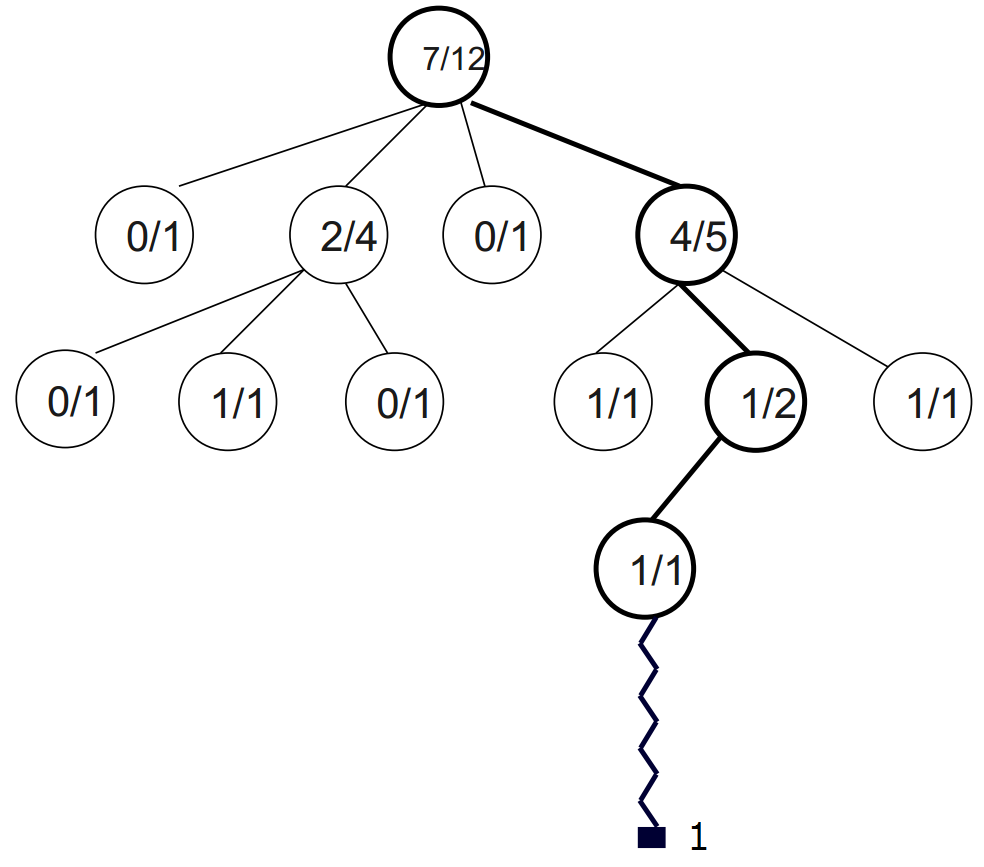
\includegraphics[height=4cm]{1_Presentation/1.2_Algorithm_MCTS_Benoit/img/12.png}
	\end{minipage}%
\end{figure}

Make a decision : here we chose the fourth leaf.\\
\newpage
\subsubsection{How to select the leaves to develop ?}
In the previous exemple, we chose to not expend leaves without winrates. But depending on the results of the simulations, wins can vary greatly. Therefore we will run more simulations on each leaf before chosing the ones to develop. For practical purpose we will select the leaves to expend that has the highest value of the cost function UCT (Upper Confidence Bound 1 applied to Trees).\\
\bigskip
\begin{minipage}[b]{1\linewidth}
\centering
\begin{equation*}
f = \frac{w_i}{n_i} + c\sqrt{\frac{\ln t}{n_i}}
\end{equation*}
\medskip
\textit{UCT function}\cite{formula_UCT}

\end{minipage}%
\bigskip
\begin{itemize}
  \item \ensuremath{w_i} : number of wins after the ith node
  \item \ensuremath{n_i} : number of simulations after the ith node
  \item \ensuremath{c}   : exploration parameter – theoretically equal to \ensuremath{\sqrt{2}} but in practice chosen empirically
  \item \ensuremath{t}   : total number of simulations in a given tree node, equal to the sum of all \ensuremath{n_i}
\end{itemize}
\medskip
The more a leaf is developed, the less it's cost is worth it. This way we can be sure that a leaf with low winrate isn't completely forgotten.\\

\subsubsection{Why using the Monte Carlo Tree Search ?}
 The advantage of MCTS with it's basic form is that you don't need to implement functions to improve the researches. Based on its random simulations, it will determine by itself which are the good options and which aren't.\\ The more you run simulations, the more accurate the results will be.

\subsubsection{How much power do we need ?}
The more the game has possible moves, the more power it require to solve. In order to get decisions, it needs to go deeper in the tree and to search enough leaves. If the time or number of simulations is not sufficient, the algorithm might miss some important branches and fail to give plausible results. Therefore in order to get decent results, using high-end computer is mandatory, it allows us to get access to multi-threading technology in order to parallelize the simulations.

\newpage
\section{Strategies and state of the art}
\subsection{Strategy of root parallelization}Now, let’s see how we can parallelize the Monte-Carlo Tree Search to optimize our algorithm. A classic MCTS is an algorithm which sequentially creates random development of the game. In order to speed up the results, develop more nodes of the tree search or even have more realistic statistics, we will parallelize our tree. It means that we will distribute parts of the tree development to multiple threads, among multiple computers. Therefore, each thread on each computer will have less executions and our algorithm will be more efficient.
\newline
\newline
Currently, there are three principal strategies about how to parallelize the tree. They are called: Leaf Parallelization, Root Parallelization and Tree Parallelization.

\subsection{Leaf Parallelization}

The Leaf Parallelization is the easiest way to parallelize the tree. In this method, only one thread traverses the tree and adds one or more nodes to the tree when the leaf node is reached. Then, all the threads will independently play the game. Once they all have finished, they back-propagate their results to the leaf and then, only one thread change the tree’s global results.
\newline
\newline
The advantage of this method is that its implementation seems very simple. There are no problems of mutual exclusions, or mutexes, between the threads. However, there are two major problems. The first one is that we don’t know the time it will take to a thread to finish the game. Therefore, it will take, in average, more time to do n games with n threads, than one game with one thread, since this method wait for the last one. The second problem is that there’s no communication between the threads. If a majority of the threads, the faster ones, have led to a loss, it will be very likely than all of them lead to a loss. And so, we will develop the last one for nothing.

\subsection{Root Parallelization}

The second method is the Root Parallelization. It consists in giving each thread the same tree during the same amount of time. They will independently and randomly develop their tree and, at the end of the time, they will merge all of the results. This method can also be called “Single-run parallelization” or “Slow-Tree Parallelization”, for instance.
\newline
\newline
Its advantage is also one of its drawbacks. Indeed, the threads don’t communicate between each other. On one hand, it means there is some redundancy is the development of the tree. Since there is no communication, multiple threads can develop the same sub-tree. On the other hand, the lack of communication increases drastically the speed of the program. Each thread executes a different tree and as they wait for the end of the time, the program does not lose time in communication between threads. Actually, the strength of this strategy lies in the little communication.

\subsection{Tree Parallelization}

Finally, the third method is called the Tree Parallelization. In this method, multiples thread share the same tree and, they can randomly choose a leaf and develop it. The main problem of this method is that multiple threads can access the same node and corrupt data given by another thread. To prevent this corruption there is two main methods proposed by Guillaume Chaslot, Mark Winands, and H. Jaap van den Herik[REFERENCE ?]. The first one is to put mutexes on the tree and the second is to implement a virtual loss.
\newline
\newline
The mutexes can be either global or local. The global mutexes block access to the whole tree when a thread is accessing it. Yet, the lock causes a major loss of time when the average of the thread’s execution is high which is often the case. The local mutexes block only the node that the thread is using in order not to block the entire tree. This method is better but still implies an important number of locking and unlocking. However, we can use fast-access mutexes and spinlocks to increase the speed of the program.
\newline
\newline
Nevertheless, according to Markus Enzenberger and Martin Müller \cite{L1}, the data which could be corrupted by the lack of mutexes are negligible compared to the speed decrease of the program, especially when the number of threads exceeds 2. Therefore, we can assume that, to be the most efficient, we can simply suppress mutexes.
\newline
\newline
The second method, the virtual loss, consists in decreasing the value of the node the first thread access. When the second thread searches a node to develop, he’ll take this node only if it’s considerably better than the others. This strategy allows nodes with high percentages of winning to be visited by multiple nodes and avoid redundancy on the other ones.

\subsection{Comparison}
\begin{figure}[!h] 
\centerline{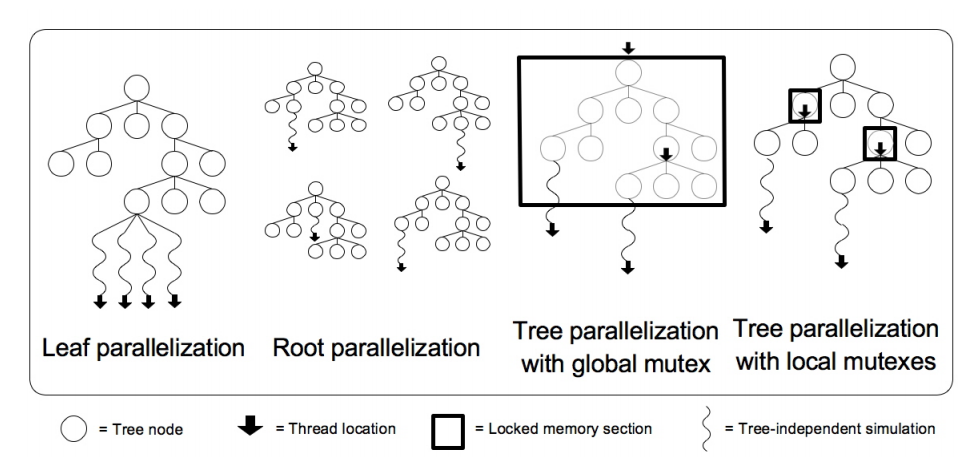
\includegraphics[scale=0.60]{2_State_of_the_art/Strategy_of_root_parallelization_Mikail/impara.png}}
   \caption{\label{étiquette} Comparison of all trees}
\end{figure}

Currently, the best strategy to adopt is the Root parallelization. According to some tests \cite{L2}, the advantages of the Root parallelization outcomes its drawbacks. Indeed, for 16 threads, a program using Root Parallelization will win 56% of the time against 36.5% for the Leaf parallelization, and 49% for the Tree parallelization with the use of a virtual loss. Moreover, the Root is always twice faster than the Tree with virtual loss. We can explain that by the fact that numerous trees are massive, and so, you will lose much time doing communication and synchronization. You don’t have any of those problems with the Root strategy. Furthermore, this method is also very simple to compute.

\subsection{Hybrid Algorithms}

Now, we can wonder if there is some research which has already be done on hybrids technologies of parallelization. Some parallelization strategies are a combination of multiples methods with some additional content, but they are very complex to compute and are efficient in specific case.  There is, for instance, the UCT-Treesplit algorithm which retake the base of Root algorithm and add to it work clusters on which compute nodes can process. It’s made for High-Performance Computers (or HPC) which have cluster parallelization and shared memory parallelization. Moreover, this method demands a lot of communication and so, the network latency is a very important factor of slow-down. 

\subsection{Conclusion}

In our case, we will also have those two types of parallelization to compute so we can use this type of algorithm. We can also choose a simple Root parallelization between the different computers, and them, use another algorithm, specialized in shared memory parallelization, within them. 

\subsection{State of the art of MCTS}Until 2002, methods based on decompositions and positions evaluations were used in order to solve such games. From 2002 to 2005 the Monte Carlo algorithm was used in order to find the best moves. Since 2006, it's implementation in a tree (MCTS) has been developped, rocketing the results in term of Artificial Intelligence on Go. On june 5th, 2013, Zen a Go programm defeated Takuto Ooomote (9 Dan) with a 3 stone handicap.\cite{computer_Go_vs_human}
\begin{figure}[H]
\centering
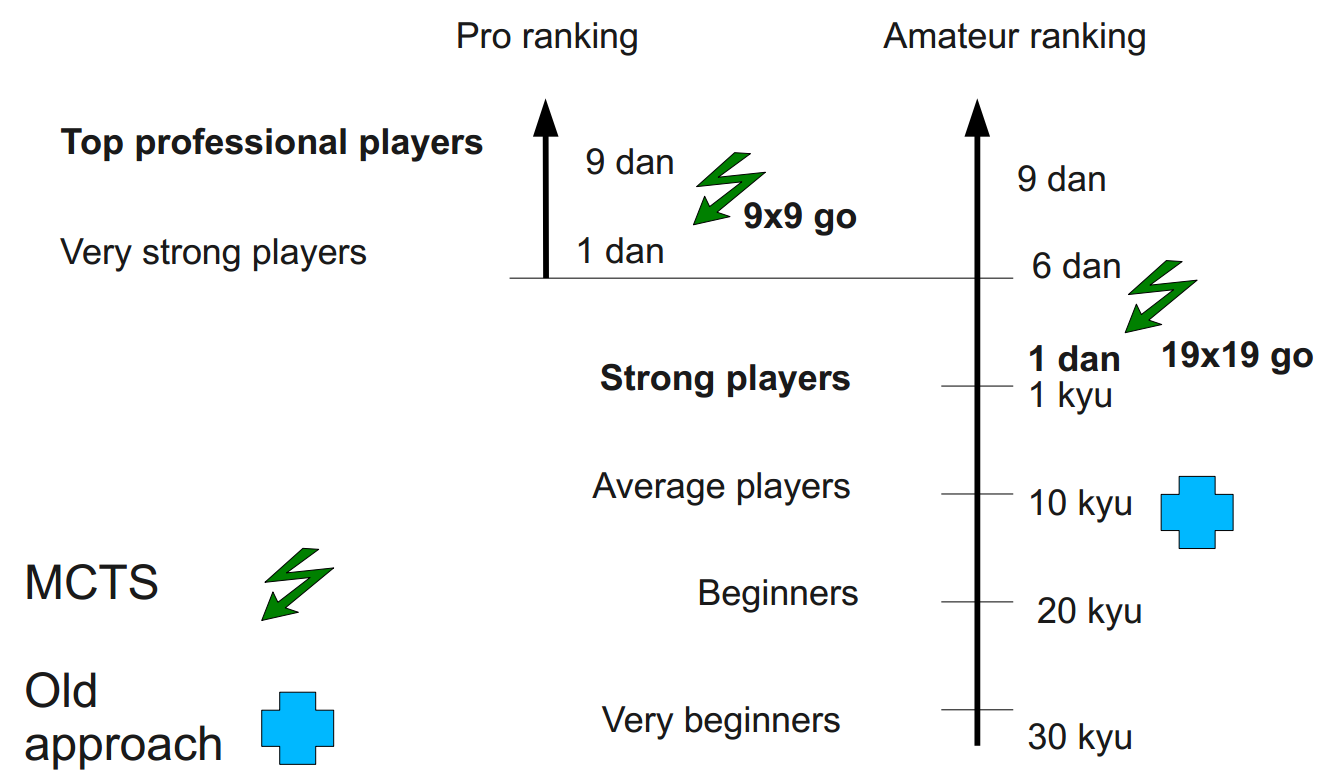
\includegraphics[width=12cm]{2_State_of_the_art/Arimaa_on_MCTS_Benoit/img/ranking.png}
\caption{\label{fig:ranking}Comparison between Go algorithms and human skill (\textit{2011})\cite{graphic_MCTS_Go}.}
\end{figure}
\textit{The ranking system of the game of Go is the following : kyu are for students ranks, Dan are masters ranks. Beginners start at 30 kyu and advance downward the kyu grades. Once one ranks over 1 kyu, he will receive the 1st Dan (as the black belt in Judo) and will move upward through the Dan ranks until the 9th.}\bigskip
\\
However MCTS wasn't the first method applied in order to solve Arimaa, the \ensuremath{\alpha\beta} method was used first. At the moment the top programms (Bomb by David Fotland : 2002 to 2008, Clueless by Jeff Bacher 2009) are ranked about 1800 elo\footnote{\textit{The Elo rating system is a method for calculating the relative skill levels of players in competitor-versus-competitor games such as chess. It use also used for Arimaa. Beginers rank around 1200 elo, experts around 2000 elo and International Masters over 2400 elo.}}. For comparison, strongest humans players are rated around 2450 elo.\cite{master_mcts_kozeleck}
\medskip


\newpage
\section{Solutions and schedule}
\subsection{Candidates software and technologies}\subsubsection{Language}

At the beginning of the project, C++ was chosen to code the software. This is for simple reasons: C++ being compiled, it is runs faster so it's more indicated than Java to create an efficient algorithm.  Moreover it has several complete graphical libraries, like \emph{Qt} and \emph{SFML}, so it's easy to create the graphical interface that will be needed for the project.

\subsubsection{Software}

The software used to develop the project has already been chosen. The coding will be realized on \emph{Microsoft visual studio 2013}, and the version manager will be git. These two softwares are used a lot in the industry so we have to be familiar with them.
For the bibliography, Zotero will be used as it allows for the creation of .bib files, the bibliographic format use by LaTeX.

\subsubsection{Grid5000}

Grid5000 is a French cluster of computers that links a lot of computers from different research centers. Some of this machines have, in addition of a good CPU, a NVIDIA Tesla GPU that could be use to parallelize the \emph{MCTS}. Of Course use this cluster will require some specific parallelization that will be introduced in the next part.

\subsubsection{Parallelization}

\paragraph{Multi cores parrelization}\mbox{}\\\mbox{}\\
OpenMp is a very simple and efficient parallelization language. It consists in some pre-compilation instructions, and with only a few lines of code it can make a parallelized version of any algorithm. But it isn't perfect: in fact, as you can see in figure \ref{fig:OpenMp}, it uses a large part of shared memory which allow a quick and efficient communication between the different threads. But it's not designed for a cluster of computers, because the memory access will be too long if this memory is used by two computers which are far away. That is why another parallelization method will have to be used for that purpose.
\begin{figure}[!h] 
\centerline{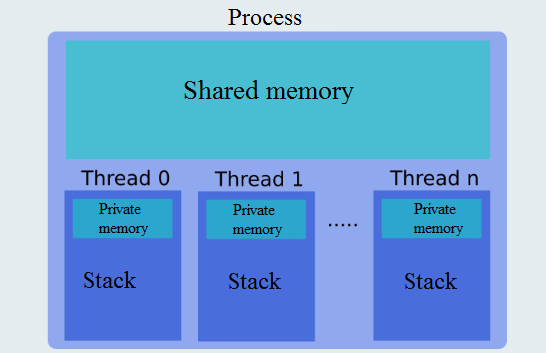
\includegraphics[scale=0.50]{3_Software_considered/MultithreadingMP_boost_Visual_MPI_5000_Zotero_Project_Baptiste/OpenMP}}
   \caption{\label{étiquette} OpenMp : memory management}
\label{fig:OpenMp}
\end{figure}
\newpage
\paragraph{Computer parallelization}\mbox{}\\\mbox{}\\

MPI is a more complex method of parallelization than openMp, but it's more complete. In addition using several cores on a single machine, we can also use MPI to design our software to use a cluster of machines. As you can seein figure \ref{fig:MPI}, it doesn't use shared memory, all the data of the threads are duplicate at their creation. It uses signals to permit the communication between the threads. One of its advantages is that it makes possible to use multiple computers, as the data are duplicated their isn't the problem of time to access the memory. But we have to pay attention to the cost of communication between the threads, if we use too much the signals we will lose all the time we can gain with the parallelization. It's very adapted for a tree parallelization, because with it we have just to duplicate the data at the beginning and return the result at the end of the assign time.

\begin{figure}[!h] 
\centerline{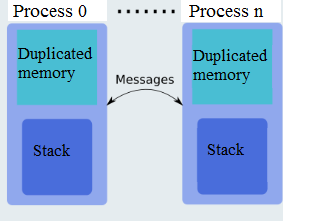
\includegraphics[scale=0.85]{3_Software_considered/MultithreadingMP_boost_Visual_MPI_5000_Zotero_Project_Baptiste/MPI}}
   \caption{\label{étiquette} MPI : memory management}
\label{fig:MPI}
\end{figure}


\paragraph{Hybrid parallelization}\mbox{}\\\mbox{}\\

As we see openMp and MPI have each one their advantage and inconvenience, but we can reduce the problems by using both. That means that we can use MPI to dispatch the work onto the different computers and after use openMp to divide it on the different threads of each machine. This can permit to use together multiples parallelization strategy like tree between the machine and leaf or root on each machine. Also it reduce the manual treatment that we have to define in the code to manage the threads. It means too that we reduce the threads interaction, so we kept a maximum of the parallel code.

\paragraph{Boost Library}\mbox{}\\\mbox{}\\

Boost is a classical library of C++ which permits, amongst other things, the management of threads, basically we can use it only for one computer but it also contains a socket handling which should easily permit a parallelization between several machines. The library seems to be simple to use and complete. Also it holds tools for Graph modelisation that can improve a lot the efficiency of our algorithms.

\paragraph{GPU implementation}\mbox{}\\\mbox{}\\

During our research we heard about using the GPU to improve the MCTS algorithms efficiency, as Kamil Rocki said in his thesis "Large Scale Monte Carlo Tree Search on GPU"  \cite{GPU} : one GPU's performance is equivalent to 50 CPU threads. But this implementation has some defaults, in fact the Gpu possess very few cache memory, so if the data model is too big the parallelization will be inefficient. Also the trees that it creates will be less deep than those of a CPU, but when a CPU can develop 2 branches a GPU will develop hundreds branches simultaneously. Another thing we have to know is that a GPU can switch to another thread immediately without any cost of context switching. 

Grid5000 has NVIDIA GPU so one of our possibility is to use hybrid as I describe previously by using MPI (or boost library) and openAcc (an equivalent of openMp which allows to use GPU) or CUBA (a framework for GPU parallelization develop by NVIDIA). In this way we should be able to develop greats trees and have a better solution compare with using only CPU, even if the trees will be less deep.
\subsection {Planning management} \label{last last part}
To manage the work on this project, MS Project will be used to record the length and assigned team member of each task.
\newline

At the start of the project, the deadlines were added to MSProject. These deadlines concern the reports (analysis, specifications, ..), the orals and the finalization of the project. After this, task assignements will be decided on a weekly basis, and be added to the planning.
\newline

For the moment no programming has been planned because the specifications are not decided yet. The programming that has been done is the creation of a model of the game and its graphical interface, for the team to play the game and to display the future results of the algorithm. This will allow us to try our hand at the game and make the implementation easier.
\newline

In the next part of this project, the specifications as well as the model for our project will be decided. Accordingly, the implementation will be planned.
\newline

Another important point is role distribution. For the moment, three specific roles have been assigned: 
\begin{itemize}
\item Gabriel is in charge of the application, who supervises the implementation.
\item Baptiste is in charge of the planning, who sets the deadlines of every task, and make sure the deadline are respected.
\item Dan is the secretary, who writes the weekly reports and organizes the meetings.
\end{itemize}

In addition to these roles, the whole team has to research the informations that is needed to realize the software. Those who do not have a special role for the moment will be responsible for one of the next reports.
\newpage
\section{Conclusion}
Finally, our project is about creating an Artificial Intelligence able to compete with others computers.
\newline
\newline
Arimaa is a two players game. It has been designed to be difficult to foresee for computers, but easy to play for humans. 
In order to realize our project, we will need some concepts and technologies. 
We will use the MonteCarlo Tree Research algorithm, to take the best decisions in our game. We will decide what move to play according to this algorithm figures. Because of the numerous moves possible, we will need to choose to develop some of the better ones, that will depend on the chosen parallelization tree. Any variation could totally change statistics.
We already analyse the state of the art of Arimaa and the MonteCarlo Tree Research. Consequently, we will base our work on these thesis, to best predict decisions, without doing what has already been done.
We already know how to play this game. So it would be easier to create strategies for our Artificial Intelligence. 
\newline
\newline
The point of this project is as well to test our program upon Grid5000, a network of multi-core machines. Then we will be able to compete with other computers, comparing algorithms and power of calculus.


\newpage
\bibliography{bibliography}
\bibliographystyle{plain}

\end{document}